%% $Id: bio_transport.tex,v 1.4 2007/02/12 22:03:06 benkirk Exp $
\chapter{Biological Transport \label{app:bio}}


%%%%%%%%%%%%%%%%%%%%%%%%%%%%%%%%%%%%%%%%%%%%%%%%%%%%%%%%%%%%%%%%%%%%%%%%%%%%%%%
\section{Radial Spots Behind an Advancing Swarm Ring}
This section presents mesh and time convergence studies performed for the biological application presented in Section~\ref{sect:swarm_ring}.  The goal of these studies was (b) to produce high-accuracy reference solutions and (b) to determine the time accuracy required for the system.  These solutions are used for comparison to validate the adaptive algorithm.

\clearpage
\subsection{Mesh Convergence}
\begin{figure}[hbtp]
  \begin{centering}
    \subfigure[Bacteria]{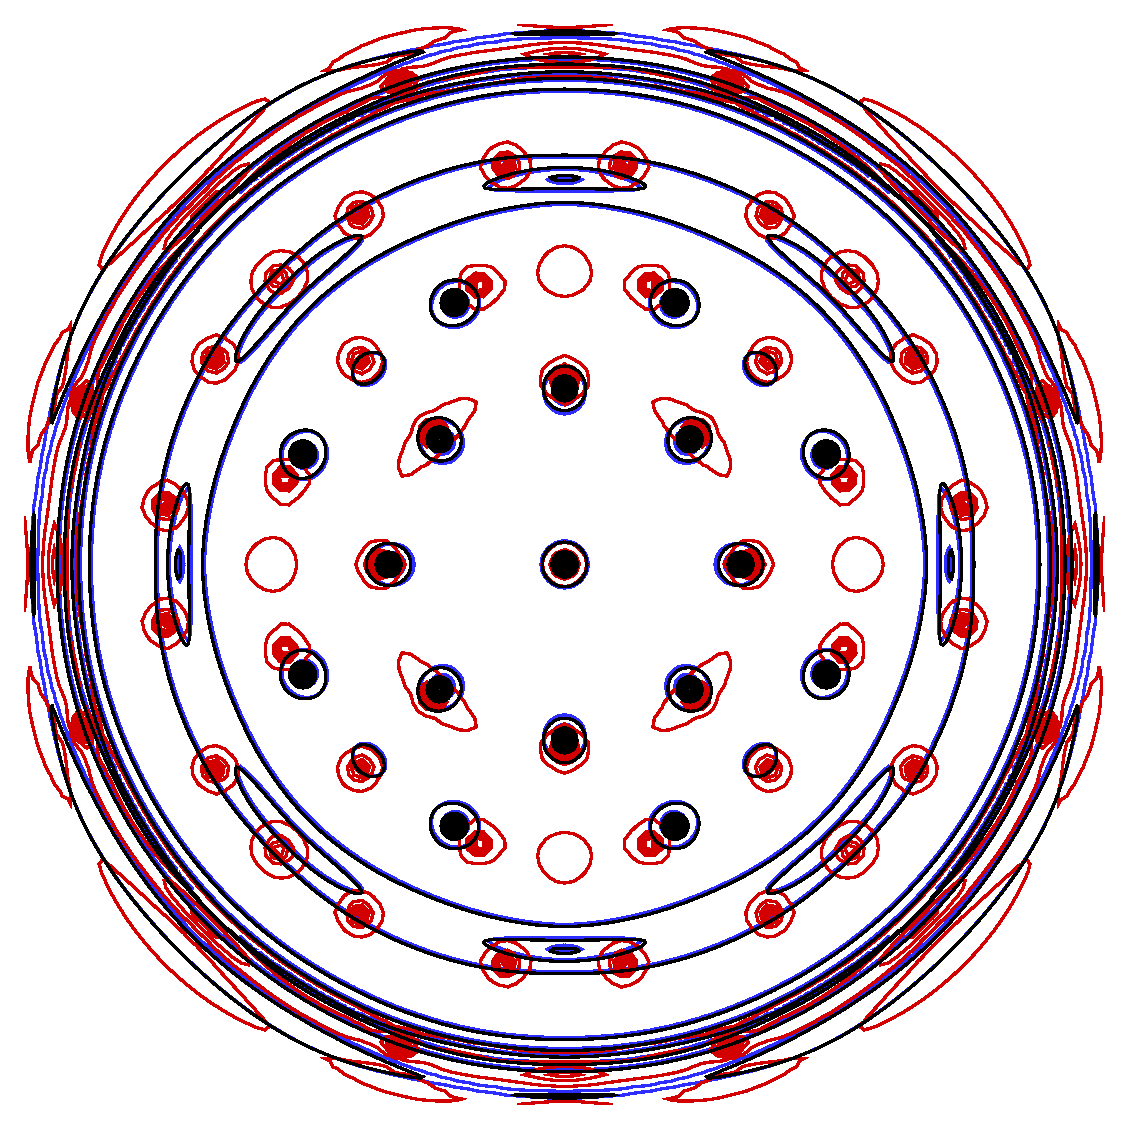
\includegraphics[height=.28\textheight]{figures/bio_radial_spots/mesh_convergence/overlay_u}} \\
    \subfigure[Chemoattractant]{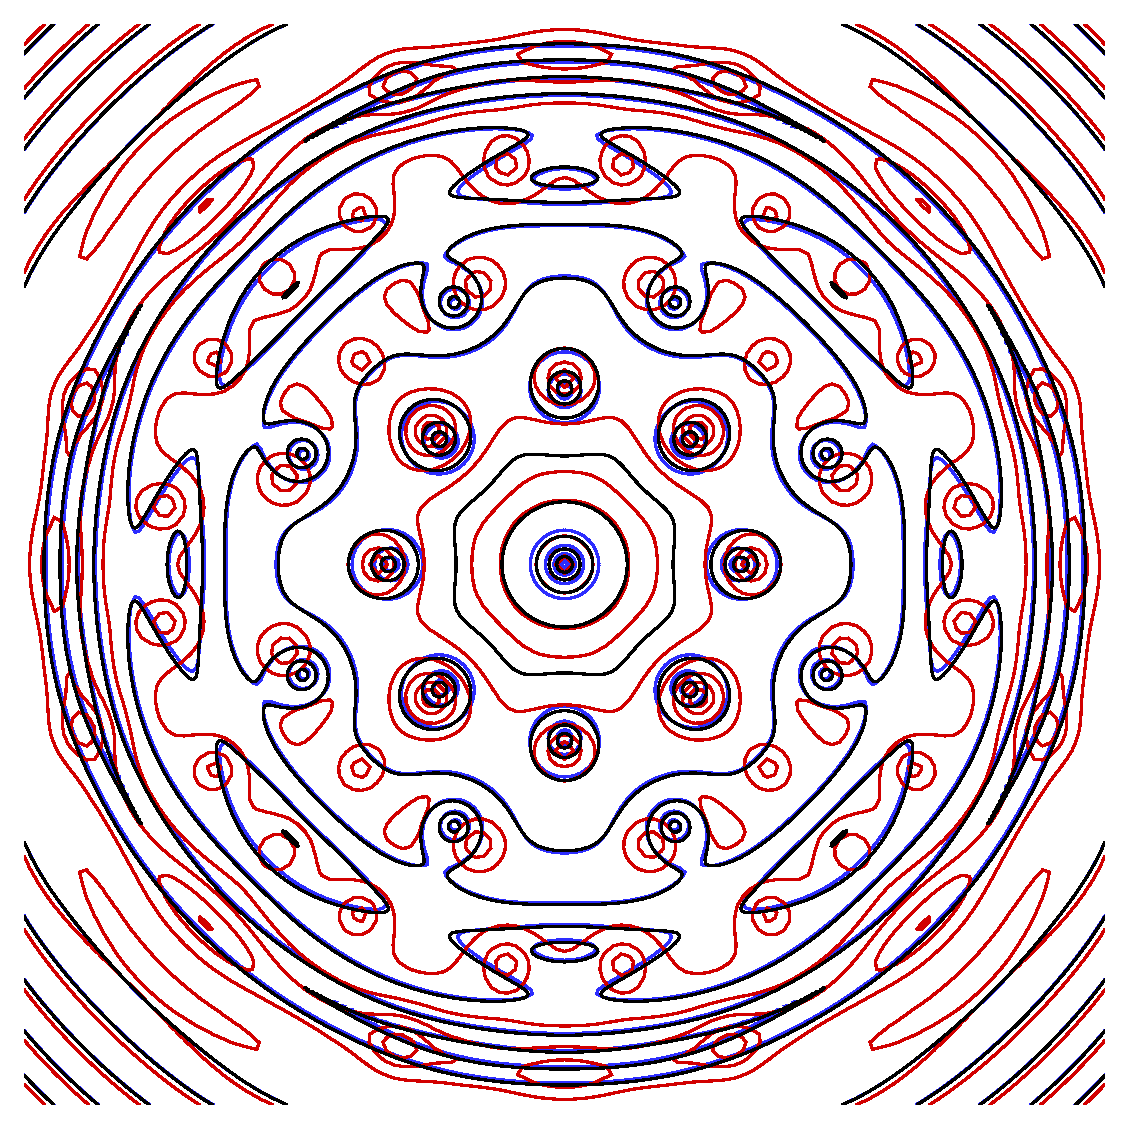
\includegraphics[height=.28\textheight]{figures/bio_radial_spots/mesh_convergence/overlay_v}}
    \caption[Overlayed concentrations at $t=19$ on illustrating mesh convergence]{Overlayed concentrations at $t=19$ illustrating mesh convergence for \textcolor{red}{$100\times 100$}, \textcolor{blue}{$200\times 200$}, and $400\times 400$ uniform meshes.  The region of interest is a $[-10,10]^2$ subdomain.  Mesh convergence is obtained for the $200\times 200$ mesh.}
  \end{centering}
\end{figure}

\clearpage
\subsection{Time Convergence}
\begin{figure}[hbtp]
  \begin{centering}
    \subfigure[Bacteria]{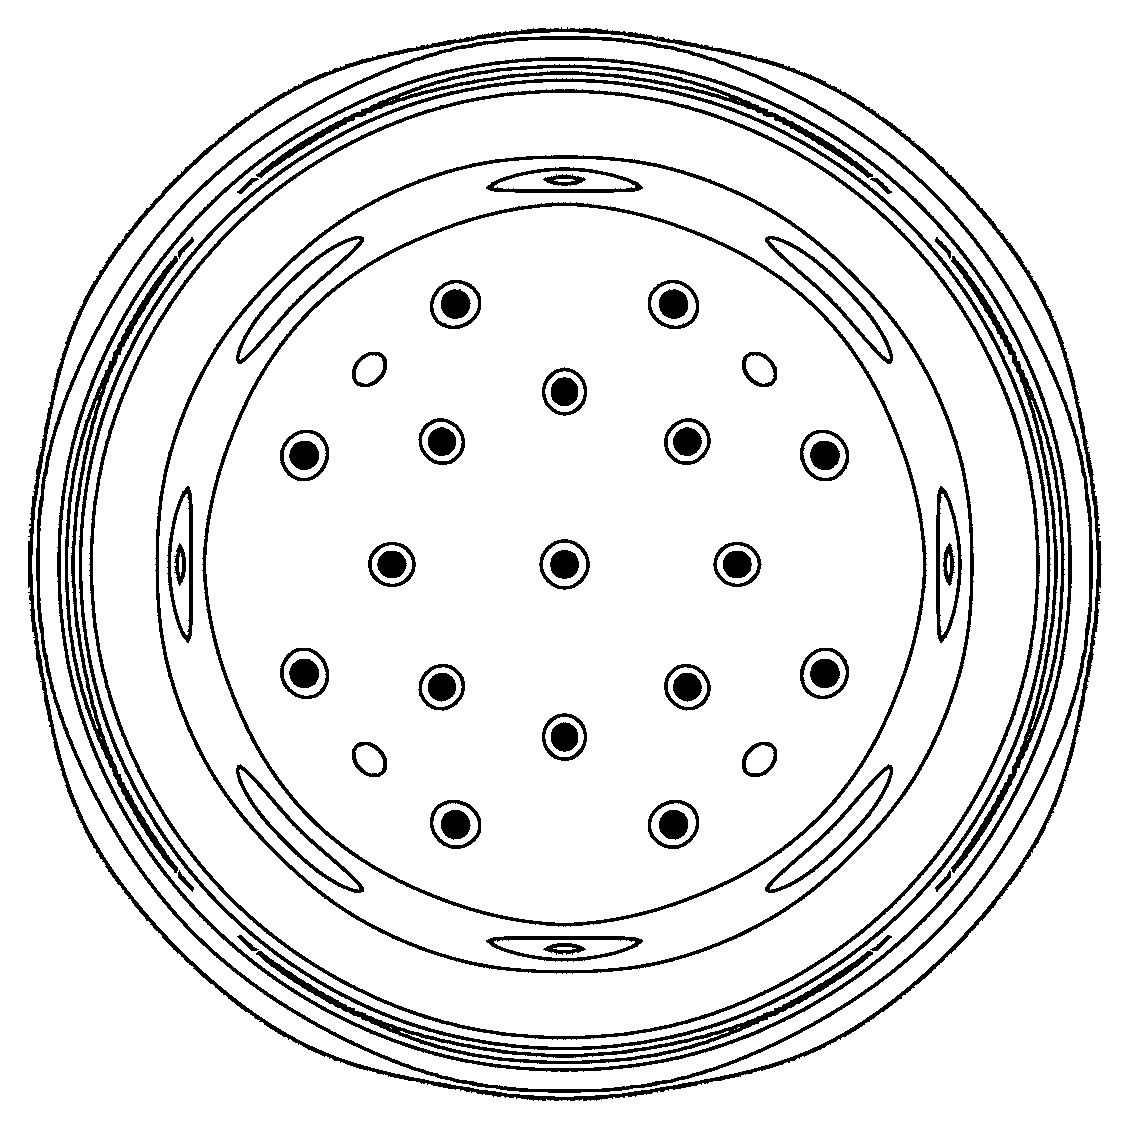
\includegraphics[height=.28\textheight]{figures/bio_radial_spots/time_convergence/quad9_200x200/overlay_u}} \\
    \subfigure[Chemoattractant]{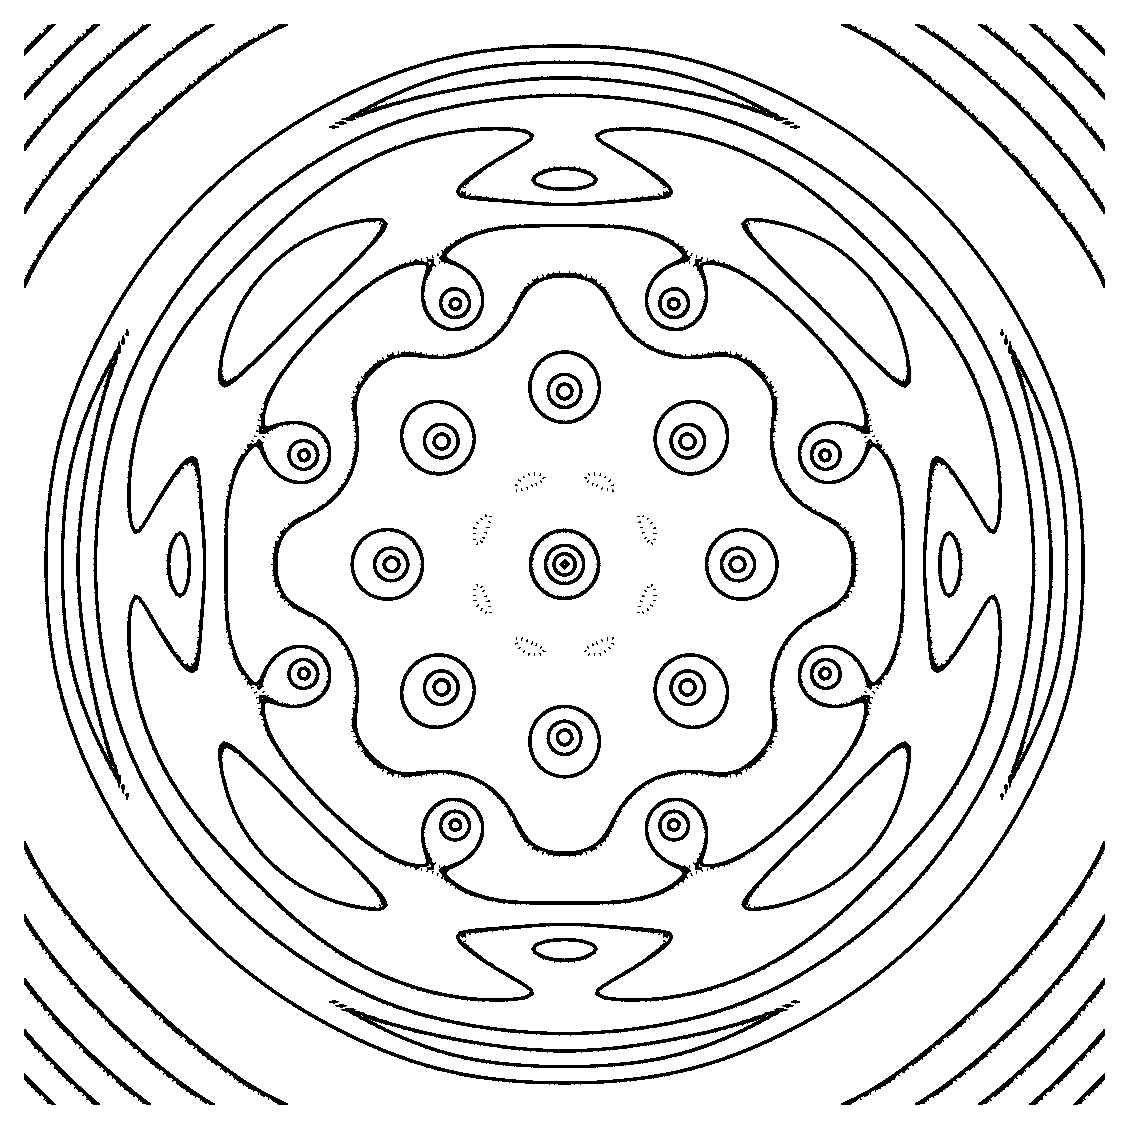
\includegraphics[height=.28\textheight]{figures/bio_radial_spots/time_convergence/quad9_200x200/overlay_v}}
    \caption[Overlayed concentrations at $t=19$ on a $200\times 200$ uniform mesh illustrating time convergence]{Overlayed concentrations at $t=19$ on a $200\times 200$ uniform mesh illustrating time convergence for $\varepsilon_t=$\textcolor{black}{$2\times 10^{-2}$}, \textcolor{black}{$1\times 10^{-2}$}, \textcolor{black}{$5\times 10^{-3}$}, and $2.5\times 10^{-3}$.  The region of interest is a $[-10,10]^2$ subdomain.  Essentially all cases are time converged.}
  \end{centering}
\end{figure}



%% Local Variables:
%% TeX-master: "dissertation.tex"
%% TeX-command-default: "Make"
%% End:
